\documentclass[handout]{beamer}
\mode<presentation>
\usepackage{beamerthemesplit}
\usepackage{amsmath}
\usepackage{amsthm}
\usepackage{amsfonts}
\usepackage[english]{babel}
\usepackage{amssymb}
\usepackage{etex}
\usepackage{xy}
\input xy
\xyoption{all}

%\uselanguage{spanish}
%\languagepath{spanish}


%\uselanguage{Spanish}
%\languagepath{Spanish}

\theoremstyle{plain}
\newtheorem{prop}{Proposici\'on}[section]
\newtheorem{teor}{Teorema}[section]
\newtheorem{defi}{Definici\'on}[section]
\newcommand{\coker}{\operatorname{coker}}
\renewcommand{\P}{\mathbb{P}}
\newcommand{\G}{\mathcal{G}}

\title{Rigidity, Mapping  Class Groups  and Stochastic Topology. }
\author{No\'e B\'arcenas.\\ Joint work with O. Arizmendi \\  and R.Ch\'avez C\'aliz.}
\institute{Centro de  Ciencias Matem\'aticas. \\ UNAM. }
\date{V Escuela  de  An\'alisis Topol\'ogico  de  Datos.}
\begin{document}
\begin{frame}
\titlepage
\end{frame}

\begin{frame}
\frametitle{Overview}
We propose the use of random topology to provide a probabilistic insight to the specific phenomena: \textbf{rigidity}.\\
For this, we will first motivate the study of rigidity in the curve complex associated to a surface, after that we can give the stochastic approach.
\end{frame}

\section{Rigidity}

\begin{frame}
\frametitle{What  is  rigidity?}

Rigidity phenomena called mathematicians attention because it \textbf{uses the structure of the objects to describe morphisms between them.}

%Examples of rigidity that you know
\end{frame}

\begin{frame}
\frametitle{Rigidity in mapping class group}

We know surfaces. \\
\begin{figure}[h!]
	\centering
	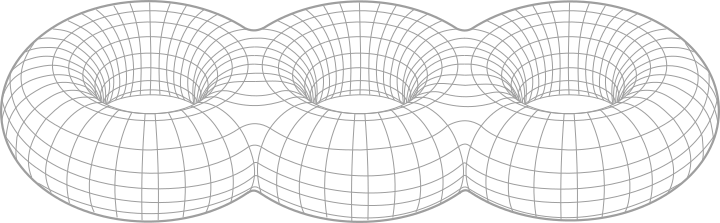
\includegraphics[scale=0.35]{CHARLA_STOCHASTIC_TOPOLOGY_MCG_CIMATNOVEMBER_2018/multitorus.png}
	\caption{Surface of genus 3}
\end{figure}

We  can  associate a  group  to the surface, $Mod(S)$,  the  mapping  class  group. \pause
Rigidity: Group  homomorphisms 
$$ Mod(S) \to Mod  (S^{'})$$
are  induced  by  manipulation  of  the  given surfaces. 
\end{frame}


\begin{frame}\frametitle{Why the mapping class group ?}

Let  $S$  be  a 2- dimensional  smooth  manifold without  boundary. \pause
$S$  can  be  furnished  with  a Riemannian  Metric, even with  a  complex structure. \pause Is  it  unique? \pause
NO. \pause 

There  is  a  \textbf{whole  space $T(S)$ of  complex  structures  on  $S$.} \pause (Homeomorphic  to  an  euclidean ball  of  dimension $6g-6$  if  the  surface  has  genus  $g$). \pause 

\end{frame}

\begin{frame}
\begin{definition}\frametitle{Mapping Class Group!.}
The  \textbf{mapping class group}, $Mod(S)$ is the  (discrete!) group  of  (orientation preserving) homeomorphisms of  the  surface, modulo  the subgroup of homeomorphisms  which  are  homotopic  to  the  identity. \pause

$$ Mod(S)= Homeo^{+}(S)\diagup Homeo_{0}(S). \pause $$
(Versions for  a  surface with  a  finite  number  of boundary  components). 
 
 \end{definition}
 \end{frame}
 


\begin{frame}\frametitle{Curve complex }
\textbf{How to understand $Mod(S)$? }\pause
Consider a  closed  surface. A  curve  $\alpha$ inside  it  is  the  image of  a  continuous  map. It  is  essential if no component of $S-\alpha$ is  a  disk.      
We  will  consider   now  the (discrete) collection of isotopy classes   of  essential  curves.

\begin{figure}[h!]
	\centering
	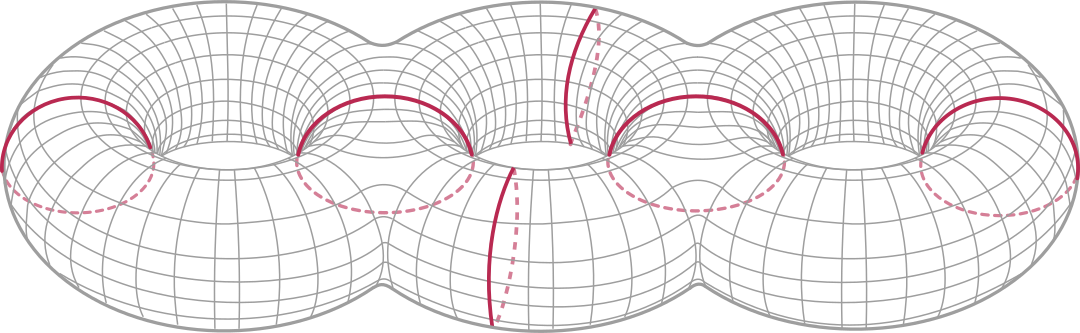
\includegraphics[scale=0.2]{CHARLA_STOCHASTIC_TOPOLOGY_MCG_CIMATNOVEMBER_2018/Pantalones.png}
	\caption{Some essential curves}
\end{figure}

\end{frame}
\begin{frame} \frametitle{The  Curve  complex!}

And  we  will  put  an edge  connecting  them  if   they  admit  a realization  without  intersection. 

\begin{figure}[h!]
	\centering
	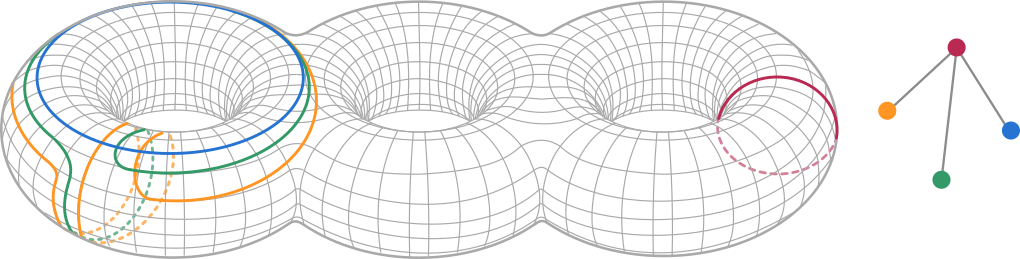
\includegraphics[scale=0.25]{CHARLA_STOCHASTIC_TOPOLOGY_MCG_CIMATNOVEMBER_2018/Locally-infinite.png}
	\caption{Construction of the curve complex}
\end{figure}

One  gets  a simplicial  (flag) complex,  denoted  by $\mathcal{C}(S)$, the  curve  complex. \pause  
\end{frame}
\begin{frame} \frametitle{Rigidity  of  the  Curve  complex}
 The mapping class group acts on the Curve complex.

\begin{theorem}[Luo]

Let  $S$  be  a  closed  surface  of  genus  at  least  $2$. The (simplicial) automorphisms  of the curve complex $\mathcal{C}$ are  in bijective correspondence  with  isotopy classes of homeomorphisms  of  the  surface.   \pause 
$$Aut(\mathcal{C}(S))\cong Mod^{*}(S).\pause $$
\end{theorem}

\end{frame}

\begin{frame}
Here, such classes  are  responsible  for  the  rigidity  phenomenon. \textbf{The  automorphisms  of  the  curve  complex  are  all geometric}.\pause  The  group  of simplicial   automorphism  of  the  curve  complex  is  the  extended  Mapping  Class group. \pause Ivanov's Rigidity  meta-conjecture.

Version  of  Margulis Superrigidity Theorem. 
 

\end{frame}


\section{Rigidity in random graphs}
\begin{frame}

Recall  the  curve  complex, $\mathcal{C}(S_g)$ is a flag complex of a \textbf{graph}. We have the following theorem

 \begin{theorem}
Let  $S_g$ be  a  genus  $g$  closed  surface, where  $g$  is t  least $2$. 
The  curve  graph  has  the  following  properties: 
\begin{itemize}
\item  It  is  connected. 
\item Every  vertex  has  infinite degree. 
\item It  has  clique  number  equal  to $3g-3$
\item It  has infinite  diameter.  
\end{itemize}
\end{theorem}
\end{frame}

\begin{frame}{Rigidity in graphs}
    \begin{definition}
Let $\Gamma$ be a simplicial graph and let $H<\Gamma$ be a vertex-induced subgraph. A function $f:y\to \Gamma$ is \textbf{locally injective} if $f|_{star(v)}$\footnote{The $star(v)$ is the vertex-induced subgraph with vertices $\{ v \} \cup N(v)$ ($v$ plus its neighborhood).} is injective for all $v \in V(y)$. 
\end{definition}

\begin{definition}
$H<\Gamma$ is \textbf{rigid} if every locally injective function defined in $H$ can be extended to an automorphism of $\Gamma$. 
\end{definition}
\end{frame}

\begin{frame}
A vertex $v \in V$ in a graph it's called to be uniquely determined by $A\subset V(G)$, denoted $v=<A>$, if $v$ is the unique neighbor of every element of $B$, i.e.

$$ \{ v \} = \bigcap_{w\in B} lnk(w) $$

\begin{definition}
The first rigid expansion of $Y\subset \Gamma$ is the vertex-induced subgraph whose vertices are
$$ V(Y) \cup \{ v\in V(\Gamma) :  \exists A \subset V(Y) \text{ where } v = <A>  \}$$
\end{definition}

\end{frame}
%\section{Main Results}
%\begin{frame}\frametitle{Explanation}

%Aim  of  this  Effort:  give  Probabilistic  proofs  of properties of  the  curve complex, based  on the  theory  of  random graphs.  \pause 
%The  easy  ones: the  four  fundamental  properties  listed above. (Nice  didactical  introduction  to  fundamental   ideas  of  random graph theory). \pause Reason to be delivered here  in the  TDA-Stochastic  topology  School. \pause   
%This  gives  probabilistic  proofs  of   results  about  mapping  class  groups.  \pause 
%\end{frame}

%\begin{frame}

%The more  involved  one, but also  adressed here: Luo's proof  of  rigidity  of  the  curve  complex.  \pause 
%\end{frame}
\section{Stochastic model}
\begin{frame}{Why Stochastic topology?}
\begin{itemize}
    \item We would like to answer the rather vague question: \textbf{How common is rigidity?}
    \item Doing rigid expansion by hand its hard
    \item There is a  whole translation of the mapping class group rigidity phenomenon in terms of random graph theory.
\end{itemize}    
\end{frame}


\begin{frame}

\textbf{Slogan: The  Curve  complex  is   very  similar  to  a Random Graph  in the  sense  of  Erd\"os-R\'enyi  with  very  specific  parameters,  obtained  in the  limit (The  Rado Graph). \pause }

Deterministic counterpart: Behring-Gaster's result. 

\end{frame}

\begin{frame}\frametitle{Aknowledgements}

\begin{center}
This  is  Ricardo Ch\'avez-C\'aliz  MSc. Thesis, in process at  UNAM. 
\end{center}

Fruitful  insights  from  Octavio Arizmendi, \pause but  also a  group  of  experts on the  curve  complex  and  mapping class  groups (around Jes\'us Hern\'andez) based  in Morelia.

\end{frame}


\begin{frame}{Rigidity calculations}
With this model in mind we have the following calculations to study rigidity phenomena.

\begin{itemize}
\item What is the probability that a vertex $v$ is uniquely determined by a set of size $k$? (Event $E_1$)
 \item What is the probability that a set of size $k$ generate a rigid expansion? (Event $E_3$)
\end{itemize}

\end{frame}

\begin{frame}{Uniquely determined vertex}

\begin{figure}[h!]
	\centering
	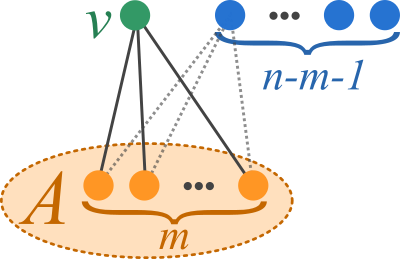
\includegraphics[scale=0.8]{CHARLA_STOCHASTIC_TOPOLOGY_MCG_CIMATNOVEMBER_2018/uni.png}
	\caption{Probability of uniquely determined vertices}
\end{figure}

If $<A> = v$ with $|A| = m$ there's a edge between $v$ and every vertex in $A$, and none of the $n-m-1$ remaining vertices is also connected to every vertex in $A$, i.e.
$$\P(E_1(m)) = p^{m}(1-p^{m})^{n-m-1}$$

\end{frame}

\begin{frame}
For the second question we have that if $A_k$ does not generate a rigid expansion is because none of the possible subsets of $A_k$ determined uniquely a vertex outside of $A_k$. 

We have that the probability that none of the vertices outside of $A_k$ is uniquely determined by $A_m\subset A_k$ is $\rho_{m,k} = (1 -  \P(E_1(m) )^{n-k}$.

$$\P(A_k \text{ generates a rigid expansion}) = 1 -  \Pi_{m=1}^{k} (\rho_{k,m})^{\binom{k}{m}}  $$

\end{frame}

\begin{frame}{Calculations}
    
\begin{figure}[h!]
	\centering
	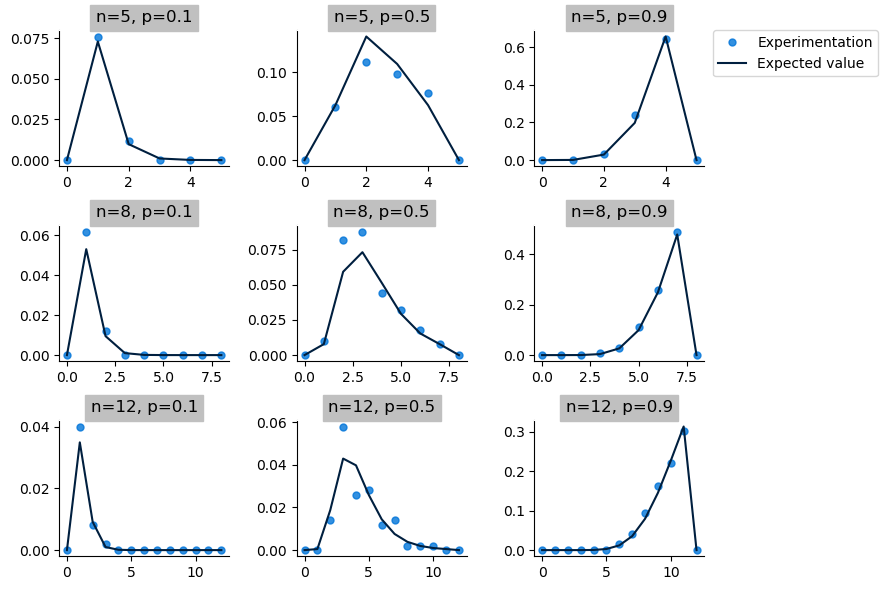
\includegraphics[scale=0.35]{CHARLA_STOCHASTIC_TOPOLOGY_MCG_CIMATNOVEMBER_2018/fixed-uniq-det.png}
	\caption{Probability of uniquely determined vertex, varying $k$ in $A_k$}
\end{figure}
\end{frame}
\begin{frame}
\begin{figure}[h!]
	\centering
	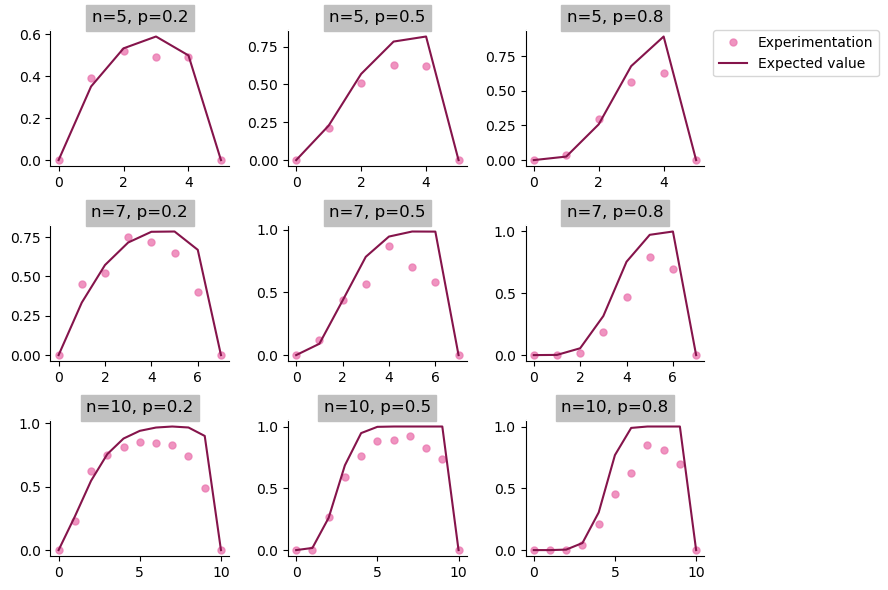
\includegraphics[scale=0.35]{CHARLA_STOCHASTIC_TOPOLOGY_MCG_CIMATNOVEMBER_2018/rig-prob.png}
	\caption{Probability of having a rigid expansion,  varying $k$ in $A_k$}
\end{figure}
\end{frame}
\begin{frame}
\frametitle{Connectedness}

\begin{theorem}
Let $\omega(n)$ be a function that tends to infinity arbitrarily slow as $n$ tends to infinity
\begin{itemize}
\item If $p\geq \frac{log(n)+ \omega(n)}{n}$ then 
$$\lim_{n \to \infty} \P(G \in \G(n,p) \text{ is connected}) = 1$$
\item If $p\leq \frac{log(n)- \omega(n)}{n}$ then
$$\lim_{n \to \infty} \P(G \in \G(n,p) \text{ is disconnected}) = 1$$
\end{itemize}
\end{theorem}

\end{frame}

\begin{frame}
\frametitle{Vertices have  infinite  degree}
\begin{theorem}
Let $\epsilon>0$ be fixed, $\epsilon n^{-3/2} \leq p = p(n) \leq 1 - \epsilon n^{-3/2}$, let $k = k(n)$ be a natural number and set $\lambda_{k} = \lambda_{k}(n) = n\cdot b(k;n - 1,p)$. Then the following assertions hold.

\begin{itemize}
\item If $\lim \lambda_{k}(n) = 0$, then $\lim P(X_{k} = 0) = 1$. 
\item If $\lim \lambda_{k}(n) = \infty$, then $\lim P(X_{k} > t) = 1$
for every fixed $t$.
\item If $0 < \lim\lambda_{k}(n) < \lim \lambda_{k}(n) < \infty$,
then $X_{k}$ has asymptotically Poisson distribution with mean $\lambda_{k}$: 
$$P(X_{k} = r) \sim e^{\lambda_{k}}\cdot \lambda_{k}^{r}/ r!$$
for every fixed $r$.
\end{itemize}
\end{theorem}
\end{frame}

\begin{frame}

\frametitle{Clique Number  and asymptotic  of  genera.}
\begin{theorem}
Let $r = r(n) = O(n^{1/3})$ and let $p=p(n)$, $0<p<1$, be such that
$$\binom{n}{r} p^{\binom{r}{2}} \to \infty \text{ and } \binom{n}{r+1} p^{\binom{r+1}{2}} \to 0 $$
Then a.e $G_{p}$ has clique number $r$
\end{theorem}
\end{frame}

\begin{frame}\frametitle{Infinite  diameter}
\begin{theorem}
Let $c$ be a positive constant, $d=d(n)\geq 2$ a natural number, and define $p=p(n,c,d), 0<p<1$, by
$$p = \frac{\big( n\cdot log(n^2/c)\big) ^{1/d}}{n}$$
Suppose that $pn/(log\text{ }n)^{3} \to \infty$. Then in $G(n,p)$ we have
$$\lim_{n\to \infty} \P (diam\text{ }G = d) = e^{-c/2} \text{ and }  \lim_{n\to \infty} \P (diam\text{ }G = d+1) = 1 - e^{-c/2}$$
\end{theorem}
\end{frame}

\begin{frame}
   \begin{center}
       Thanks!
   \end{center} 
\end{frame}

\end{document}

